% Options for packages loaded elsewhere
\PassOptionsToPackage{unicode}{hyperref}
\PassOptionsToPackage{hyphens}{url}
%
\documentclass[
]{article}
\usepackage{lmodern}
\usepackage{amssymb,amsmath}
\usepackage{ifxetex,ifluatex}
\ifnum 0\ifxetex 1\fi\ifluatex 1\fi=0 % if pdftex
  \usepackage[T1]{fontenc}
  \usepackage[utf8]{inputenc}
  \usepackage{textcomp} % provide euro and other symbols
\else % if luatex or xetex
  \usepackage{unicode-math}
  \defaultfontfeatures{Scale=MatchLowercase}
  \defaultfontfeatures[\rmfamily]{Ligatures=TeX,Scale=1}
\fi
% Use upquote if available, for straight quotes in verbatim environments
\IfFileExists{upquote.sty}{\usepackage{upquote}}{}
\IfFileExists{microtype.sty}{% use microtype if available
  \usepackage[]{microtype}
  \UseMicrotypeSet[protrusion]{basicmath} % disable protrusion for tt fonts
}{}
\makeatletter
\@ifundefined{KOMAClassName}{% if non-KOMA class
  \IfFileExists{parskip.sty}{%
    \usepackage{parskip}
  }{% else
    \setlength{\parindent}{0pt}
    \setlength{\parskip}{6pt plus 2pt minus 1pt}}
}{% if KOMA class
  \KOMAoptions{parskip=half}}
\makeatother
\usepackage{xcolor}
\IfFileExists{xurl.sty}{\usepackage{xurl}}{} % add URL line breaks if available
\IfFileExists{bookmark.sty}{\usepackage{bookmark}}{\usepackage{hyperref}}
\hypersetup{
  pdftitle={Problem Set 1},
  pdfauthor={Jake Underland},
  hidelinks,
  pdfcreator={LaTeX via pandoc}}
\urlstyle{same} % disable monospaced font for URLs
\usepackage[margin=1in]{geometry}
\usepackage{color}
\usepackage{fancyvrb}
\newcommand{\VerbBar}{|}
\newcommand{\VERB}{\Verb[commandchars=\\\{\}]}
\DefineVerbatimEnvironment{Highlighting}{Verbatim}{commandchars=\\\{\}}
% Add ',fontsize=\small' for more characters per line
\usepackage{framed}
\definecolor{shadecolor}{RGB}{248,248,248}
\newenvironment{Shaded}{\begin{snugshade}}{\end{snugshade}}
\newcommand{\AlertTok}[1]{\textcolor[rgb]{0.94,0.16,0.16}{#1}}
\newcommand{\AnnotationTok}[1]{\textcolor[rgb]{0.56,0.35,0.01}{\textbf{\textit{#1}}}}
\newcommand{\AttributeTok}[1]{\textcolor[rgb]{0.77,0.63,0.00}{#1}}
\newcommand{\BaseNTok}[1]{\textcolor[rgb]{0.00,0.00,0.81}{#1}}
\newcommand{\BuiltInTok}[1]{#1}
\newcommand{\CharTok}[1]{\textcolor[rgb]{0.31,0.60,0.02}{#1}}
\newcommand{\CommentTok}[1]{\textcolor[rgb]{0.56,0.35,0.01}{\textit{#1}}}
\newcommand{\CommentVarTok}[1]{\textcolor[rgb]{0.56,0.35,0.01}{\textbf{\textit{#1}}}}
\newcommand{\ConstantTok}[1]{\textcolor[rgb]{0.00,0.00,0.00}{#1}}
\newcommand{\ControlFlowTok}[1]{\textcolor[rgb]{0.13,0.29,0.53}{\textbf{#1}}}
\newcommand{\DataTypeTok}[1]{\textcolor[rgb]{0.13,0.29,0.53}{#1}}
\newcommand{\DecValTok}[1]{\textcolor[rgb]{0.00,0.00,0.81}{#1}}
\newcommand{\DocumentationTok}[1]{\textcolor[rgb]{0.56,0.35,0.01}{\textbf{\textit{#1}}}}
\newcommand{\ErrorTok}[1]{\textcolor[rgb]{0.64,0.00,0.00}{\textbf{#1}}}
\newcommand{\ExtensionTok}[1]{#1}
\newcommand{\FloatTok}[1]{\textcolor[rgb]{0.00,0.00,0.81}{#1}}
\newcommand{\FunctionTok}[1]{\textcolor[rgb]{0.00,0.00,0.00}{#1}}
\newcommand{\ImportTok}[1]{#1}
\newcommand{\InformationTok}[1]{\textcolor[rgb]{0.56,0.35,0.01}{\textbf{\textit{#1}}}}
\newcommand{\KeywordTok}[1]{\textcolor[rgb]{0.13,0.29,0.53}{\textbf{#1}}}
\newcommand{\NormalTok}[1]{#1}
\newcommand{\OperatorTok}[1]{\textcolor[rgb]{0.81,0.36,0.00}{\textbf{#1}}}
\newcommand{\OtherTok}[1]{\textcolor[rgb]{0.56,0.35,0.01}{#1}}
\newcommand{\PreprocessorTok}[1]{\textcolor[rgb]{0.56,0.35,0.01}{\textit{#1}}}
\newcommand{\RegionMarkerTok}[1]{#1}
\newcommand{\SpecialCharTok}[1]{\textcolor[rgb]{0.00,0.00,0.00}{#1}}
\newcommand{\SpecialStringTok}[1]{\textcolor[rgb]{0.31,0.60,0.02}{#1}}
\newcommand{\StringTok}[1]{\textcolor[rgb]{0.31,0.60,0.02}{#1}}
\newcommand{\VariableTok}[1]{\textcolor[rgb]{0.00,0.00,0.00}{#1}}
\newcommand{\VerbatimStringTok}[1]{\textcolor[rgb]{0.31,0.60,0.02}{#1}}
\newcommand{\WarningTok}[1]{\textcolor[rgb]{0.56,0.35,0.01}{\textbf{\textit{#1}}}}
\usepackage{graphicx,grffile}
\makeatletter
\def\maxwidth{\ifdim\Gin@nat@width>\linewidth\linewidth\else\Gin@nat@width\fi}
\def\maxheight{\ifdim\Gin@nat@height>\textheight\textheight\else\Gin@nat@height\fi}
\makeatother
% Scale images if necessary, so that they will not overflow the page
% margins by default, and it is still possible to overwrite the defaults
% using explicit options in \includegraphics[width, height, ...]{}
\setkeys{Gin}{width=\maxwidth,height=\maxheight,keepaspectratio}
% Set default figure placement to htbp
\makeatletter
\def\fps@figure{htbp}
\makeatother
\setlength{\emergencystretch}{3em} % prevent overfull lines
\providecommand{\tightlist}{%
  \setlength{\itemsep}{0pt}\setlength{\parskip}{0pt}}
\setcounter{secnumdepth}{-\maxdimen} % remove section numbering
\usepackage{amsmath}

\title{Problem Set 1}
\usepackage{etoolbox}
\makeatletter
\providecommand{\subtitle}[1]{% add subtitle to \maketitle
  \apptocmd{\@title}{\par {\large #1 \par}}{}{}
}
\makeatother
\subtitle{ECON 21020 Spring, 2021}
\author{Jake Underland}
\date{2021-07-06}

\begin{document}
\maketitle

{
\setcounter{tocdepth}{2}
\tableofcontents
}
\hypertarget{question-1}{%
\section{Question 1}\label{question-1}}

\hypertarget{exercise-4}{%
\subsection{Exercise 4}\label{exercise-4}}

\textit{For a randomly selected county in the United States, let $X$ represent the proportion of adults over age 65 who are employed, or the elderly employment rate. Then, $X$ is restricted to a value between zero and one. Suppose that the cumulative distribution function for $X$ is given by $F(x) = 3x^2 - 2x^3$ for $0 \leq x \leq 1$. Find the probability that the elderly employment rate is at least $.6(60\%)$}.

\begin{Shaded}
\begin{Highlighting}[]
\NormalTok{F_}\DecValTok{1}\NormalTok{ <-}\StringTok{ }\ControlFlowTok{function}\NormalTok{(x)\{}
\NormalTok{  a =}\StringTok{ }\DecValTok{3}\OperatorTok{*}\NormalTok{x}\OperatorTok{^}\DecValTok{2} \OperatorTok{-}\StringTok{ }\DecValTok{2}\OperatorTok{*}\NormalTok{x}\OperatorTok{^}\DecValTok{3}
  \KeywordTok{return}\NormalTok{(a)}
\NormalTok{\}}
\KeywordTok{F_1}\NormalTok{(}\FloatTok{0.6}\NormalTok{)}
\end{Highlighting}
\end{Shaded}

\begin{verbatim}
## [1] 0.648
\end{verbatim}

\[ \begin{aligned}
P(X \geq 0.6) &= 1 - P(X<0.6) \\
&= 1 - F(0.6) \\
&= 1 - 0.648 \\
&= 0.352
\end{aligned}\]

\hypertarget{exercise-7}{%
\subsection{Exercise 7}\label{exercise-7}}

\textit{If a basketball player is a $74\%$ free throw shooter, then, on average, how many free throws will he or she make in a game with eight free throw attemtps?}

The throws are distributed according to a Binomial distribution where
the number of free throws made is \(X\sim Bin(8, 0.74)\). Thus, the
expected value is \(np\).

\begin{Shaded}
\begin{Highlighting}[]
\CommentTok{# E[X] = np }
\DecValTok{8} \OperatorTok{*}\StringTok{ }\FloatTok{0.74}
\end{Highlighting}
\end{Shaded}

\begin{verbatim}
## [1] 5.92
\end{verbatim}

\hypertarget{exercise-10}{%
\subsection{Exercise 10}\label{exercise-10}}

\textit{Suppose that at a large university, college grade point average, $GPA$, and SAT score, $SAT$, are related by the conditional expectation $E(GPA|SAT) = .70 + .002SAT.$}

(i).
\textit{Find the expected $GPA$ when $SAT = 800$. Find $E(GPA|SAT=1400)$. Comment on the difference.}

\begin{Shaded}
\begin{Highlighting}[]
\NormalTok{E_gpa <-}\StringTok{ }\ControlFlowTok{function}\NormalTok{(sat)\{}
\NormalTok{  e =}\StringTok{ }\FloatTok{.70} \OperatorTok{+}\StringTok{ }\FloatTok{.002} \OperatorTok{*}\StringTok{ }\NormalTok{sat}
  \KeywordTok{return}\NormalTok{(e)}
\NormalTok{\}}
\end{Highlighting}
\end{Shaded}

\begin{Shaded}
\begin{Highlighting}[]
\KeywordTok{cat}\NormalTok{(}\StringTok{" E(GPA|SAT=800) ="}\NormalTok{, }\KeywordTok{E_gpa}\NormalTok{(}\DecValTok{800}\NormalTok{), }\StringTok{"}\CharTok{\textbackslash{}n}\StringTok{"}\NormalTok{,}
    \StringTok{"E(GPA|SAT=1400) ="}\NormalTok{, }\KeywordTok{E_gpa}\NormalTok{(}\DecValTok{1400}\NormalTok{), }\StringTok{"}\CharTok{\textbackslash{}n}\StringTok{"}\NormalTok{, }
    \StringTok{"Difference:"}\NormalTok{, }\KeywordTok{abs}\NormalTok{(}\KeywordTok{E_gpa}\NormalTok{(}\DecValTok{800}\NormalTok{) }\OperatorTok{-}\StringTok{ }\KeywordTok{E_gpa}\NormalTok{(}\DecValTok{1400}\NormalTok{)))}
\end{Highlighting}
\end{Shaded}

\begin{verbatim}
##  E(GPA|SAT=800) = 2.3 
##  E(GPA|SAT=1400) = 3.5 
##  Difference: 1.2
\end{verbatim}

Expected value of GPA is higher when the student's SAT score is high.

(ii).
\textit{If the average $SAT$ in the university is $1100$, what is the average $GPA$?}

\[\begin{aligned} 
E[GPA] &= E[E[GPA|SAT]] \\
&= E[.70 + .002SAT] \\
&= .70 + .002E[SAT] \\
&= .70 + .002 * 1100 \\
&= 2.9
\end{aligned}\]

(iii).
\textit{If a student's SAT score is $1100$, does this mean he or she will have the GPA found in part (ii)?}

If a student has an SAT score of 1100, they will be likely to have a GPA
in the neighborhood of 2.9, as found in (ii). However, since expected
values are probabilistic, this does not mean that all student's with an
SAT score of 1100 have the above GPA.

\hypertarget{exercise-11}{%
\subsection{Exercise 11}\label{exercise-11}}

\begin{enumerate} 
\item[(i)]  \textit{Let $X$ be a random variable taking on the values $-1$ and $1$, each with probability $1/2$. Find $E(X)$ and $E(X^2)$}  
  
\[\begin{aligned} 
E(X) &= 1 * 1/2 + -1 * 1/2 = 0 \\
E(X^2) &= 1^2 * 1/2 + (-1)^2 * 1/2 \\
&= 1/2 + 1/2 \\
&= 1
\end{aligned}\]

\item[(ii)]  \textit{Now let $X$ be a random variable taking on the values $1$ and $2$, each with probability $1/2$. Find $E(X)$ and $E(1/X)$}  
  
\[\begin{aligned} 
E(X) &= 1 * 1/2 + 2 * 1/2 = 3/2 \\
E(1/X) &= 1/1 * 1/2 + 1/2 * 1/2 \\
&= 1/2 + 1/4 \\
&= 3/4
\end{aligned}\]

\item[(iii)] \textit{Conclude from parts (i) and (ii) that, in general, $E[g(X)] \neq g(E[X])$ for a nonlinear function $g(\cdot)$.}  
  
From part (i),
\[\begin{aligned}
E[(X^2)] &= 1 \\
E[X]^2 &= 0
\end{aligned}\]  

From part (ii),
\[\begin{aligned}
E[(1/X)] &= 3/4 \\
1/E[X] &= 2/3
\end{aligned}\]

Thus, we have two examples that show that when a function $g(\cdot)$ is nonlinear, $E[g(X)] \neq g(E[X])$.  
  
\item[(iv)] \textit{Given the definition of the $F$ random variable, show that $$E(F) = E[\frac{1}{(X_2/k_2)}].$$ Can you conclude that $E(F) = 1$?}  

\end{enumerate}

\[\begin{aligned} 
E(F) &= E[\frac{X_1/k_1}{X_2/k_2}] \\
&= E[\frac{X_1}{X_2}\frac{k_2}{k_1}] \\
&= \frac{k_2}{k_1}E[\frac{X_1}{X_2}] \\
&= \frac{k_2}{k_1}E[X_1]E[\frac{1}{X_2}]\dots (Independence) \\
&=  \frac{k_2}{k_1}k_1E[\frac{1}{X_2}] \\
&= k_2 E[\frac{1}{X_2}] \\
&= E[\frac{1}{(X_2/k_2)}] \dots (Linearity)
\end{aligned}\]

We cannot conclude that \(E(F) = 1\), because \[\begin{aligned} 
E[\frac{1}{(X_2/k_2)}] &= k_2 E[\frac{1}{X_2}] \\
\end{aligned}\]\\
but, in general, \(E[g(X)] \neq g(E[X])\), so
\[E[\frac{1}{X_2}] \neq 1/E[X_2] = 1/k_2\]. Thus,
\[k_2 E[\frac{1}{X_2}] \neq k_2 \cdot 1/k_2 = 1\].

\hypertarget{question-2}{%
\section{Question 2}\label{question-2}}

\textit{Let $X$ be a random variable. Show that $Var (X) \geq 0$ using Jensen’s inequality. Can $Var (X) = 0$?}

\[\begin{aligned} 
Var(X) = E[X^2] - E[X]^2 
\end{aligned}\]\\
Since \(g(x) = x^2\) is convex, from Jensen's Inequality,
\[\begin{aligned} 
E[X^2] &\geq E[X]^2 \\
\implies E[X^2] - E[X]^2 &\geq 0 \\
\implies Var(X) &\geq 0
\end{aligned}\]

\(Var(X) = 0\), in the discrete case, implies below \[\begin{aligned}
&\Sigma_x (x -E[X])^2 = 0 \\
\implies &\forall x \in X, x = E[X] 
\end{aligned}\]

We can reach the same conclusion through analogous reasoning for the
continuous case. Thus, \(Var(X)\) can equal \(0\), and when it does,
\(p(X = E[X]) = 1\).

\hypertarget{question-3}{%
\section{Question 3}\label{question-3}}

\break

\hypertarget{question-4}{%
\section{Question 4}\label{question-4}}

\textit{Show that for random variables $(Y,X)$, $Var(Y) = E(Var(Y|X))+Var(E(Y|X))$. Explain why $V ar (Y ) \neq E (V ar (Y |X))$ using an example. Taking $X$ to be a binary variable might be easiest.}
\begin{align*}
Var(Y) &= E[Y^2] - E[Y]^2 \\
E[Y^2] &= E[E[Y^2|X]] \dots \textit{(Law of iterated expectations)} \\
&= E[E[Y^2|X] - E[Y|X]^2 + E[Y|X]^2] \\
&= E[Var(Y|X) + E[Y|X]^2] \\
&= E[Var(Y|X)] + E[E[Y|X]^2] \\
\implies Var(Y) &= E[Y^2] - E[Y]^2 \\
&= E[Var(Y|X)] + E[E[Y|X]^2] - E[Y]^2 \\
&= E[Var(Y|X)] + E[E[Y|X]^2] - E[E[Y|X]]^2 \dots \textit{(Law of iterated expectations)} \\
&= E[Var(Y|X)] + Var(E[Y|X]) \tag{1}
\end{align*}

Now, we examine the case of \(Var(Y) \neq E[Var(Y|X)]\). Take \(X\) to
be a Bernoulli variable taking the values \(0\) and \(1\). Then, from
\((1)\), \[Var(Y) \neq E[Var(Y|X)] \implies Var(E[Y|X]) \neq 0\]
\(Var(E[Y|X]) \neq 0\) implies that all values of \(E[Y|X]\) cannot be
equal, and thus \(E[Y|X=0] \neq E[Y|X=1]\). This condition implies
dependence between \(X\) and \(Y\), since for independence, we must have
\(E[Y|X=x] = E[Y] = E[E[Y|X]]\) for all \(x \in X\).

\hypertarget{question-5}{%
\section{Question 5}\label{question-5}}

\textit{Let $X \sim Bernoulli(p)$. Define $Z = 2^X − 1$.}\\

\begin{enumerate}
\item[a)] \textit{Is $Z$ a random variable? Why? What is the distribution of $Z$?}  
  
The values of $Z$ are contingent on the values of $X$, which is a random variable, thus making $Z$ also a random variable. Since $X$ takes a value of $1$ at probability $p$ and $0$ at probability $1-p$, $Z$ takes the following values:
\[Z = \begin{cases}\begin{aligned}2^1 - 1 = 1 \dots &p \\
2^0 - 1 = 0 \dots &1-p \end{aligned}
\end{cases} \]
Therefore, we can see that $Z$ has a distribution that follows Bernoulli$(p)$, and is distributed identically and dependent on $X$.  

\item[b)] \textit{Show that $E(Z) = p$}  
  
\[E(Z) = p \cdot 1 + (1-p) \cdot 0 = p\]

\item[c)] \textit{Show that $E(Z^2) = p$}  
  
\[E(Z^2) = p \cdot 1^2 + (1-p) \cdot 0^2 = p\]

\item[d)] \textit{What is $Var(Z)$?}  
  
\[\begin{aligned} 
Var(Z) &= E(Z^2) - E(Z)^2 \\
&= p - p^2 \\
&= p(1-p)
\end{aligned}\]
  
\end{enumerate}

\hypertarget{question-6}{%
\section{Question 6}\label{question-6}}

\textit{Suppose $X\sim Unif[−1,1]$, and let $Y =X^2$. Show that $Cov(X,Y)=0$, but that $X$ and $Y$ are not independent.}

\[\begin{aligned} 
Cov(X,Y) &= E[XY] - E[X]E[Y] \\
&= \int_{x=-1} ^1 x \cdot x^2 f_x(x) dx  - 0 \cdot E[Y]\\
&= \int_{x=-1} ^1 \frac{x^3}{2} dx \\
&= [\frac{1}{8} x^4]^1 _{-1} \\
&= 0
\end{aligned}\]

Thus, we see that the covariance of \(X, Y\) is \(0\). However, from the
following plot illustrating \(Y\) and \(X\), it is apparent that the two
are not independent.

\begin{Shaded}
\begin{Highlighting}[]
\NormalTok{Y <-}\StringTok{ }\ControlFlowTok{function}\NormalTok{(x) x}\OperatorTok{^}\DecValTok{2}
\NormalTok{X <-}\StringTok{ }\KeywordTok{c}\NormalTok{(}\OperatorTok{-}\DecValTok{1}\NormalTok{, }\DecValTok{1}\NormalTok{)}
\KeywordTok{plot}\NormalTok{(Y, X, }\DataTypeTok{xlab =} \StringTok{"X"}\NormalTok{)}
\end{Highlighting}
\end{Shaded}

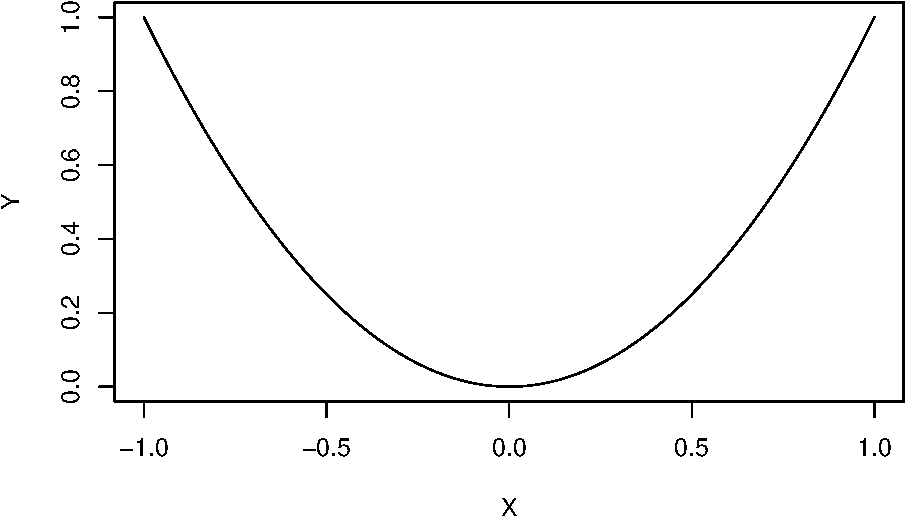
\includegraphics{Pset1_files/figure-latex/unnamed-chunk-6-1.pdf}

For a more mathematical proof, since \(Y = X^2\), we know that
\(E[Y|X = x] = x^2\). However, \[\begin{aligned} 
E[Y] &= E_X[E_{Y|X}[Y|X]] \\
&= \int _x E_{Y|X}[Y|X=x] \cdot f_x(x) dx\\
&= \int _{x = -1} ^{1} x^2 \cdot \frac{1}{2} dx \\
&= [\frac{1}{6}x^3]^1 _ {-1} \\
&= \frac{1}{3}
\end{aligned}\] Thus, for example,
\(E[Y|X=0] = 0 \neq \frac{1}{3} = E[Y]\) and thus \(Y\) is not mean
independent of \(X\), meaning they cannot be independent.

\hypertarget{question-7}{%
\section{Question 7}\label{question-7}}

\textit{Let $Y = a + bX + U$, where $X$ and $U$ are random variables and $a$ and $b$ are constants. Assume that $E(U|X)=0$ and $Var(U|X)=X^2$.}

\begin{enumerate}
\item[(a)] \textit{Is $Y$ a random variable? Why?}  
  
Yes, $Y$ is a random variable because it is dependent on the values of two random variables, each with their own probabilistic distributions. 

\item[(b)] \textit{Is $U$ mean independent of $X$? Why? Is $U$ independent of $X$? Why?}  
  
First, 
\[\begin{aligned} 
E[U] &= E[E[U|X]] \\
&= E[0] \\
&= 0
\end{aligned}\]
Furthermore, 
$$E[U|X] = 0$$
Hence, 
$$E[U] = E[U|X] =0$$
Therefore, $U$ is mean independent of $X$. However, this does not imply that $U$ is independent of $X$. In fact, since, as we show in (d), $Var(U|X) = X^2$ and $Var(U) = E(X^2)$, we see that some features of $U$ are determined by $X$, which would suggest dependency. 

\item[(c)] \textit{Show that $E(U)=0$ and $Var(U)=E(X^2)$ .}
  
We have already shown above that $E(U) = 0$.  
For $Var(U)$, 
\[\begin{aligned}
Var(U) &= E(Var(U|X))+Var(E(U|X)) \\
&= E[X^2] + Var(0) \\
&= E[X^2] + 0 \\
&= E[X^2]
\end{aligned}\]  
  
\item[(d)] \textit{Show that $ E (Y|X) = a + bX$, and that $E (Y) = a + bE (X)$.}  
  
\[\begin{aligned}
E(Y|X) &= E[a + bX + U | X] \\
&= a + bE[X|X] + E[U|X] \dots \textit{(Linearity)} \\
&= a + bX + 0 \\
&= a + bX \\
\\
E(Y) &= E(E(Y|X)) \\
&= E(a + bX) \\
&= a + bE(X) \dots \textit{(Linearity)}
\end{aligned}\] 
  
  
\item[(e)] \textit{Show that $Var(Y|X)=X^2$, and that $Var(Y)=b^2 Var(X)+E(X^2)$.}  
  
$$\begin{aligned}
Var(Y|X) &= E(Y^2|X) - E(Y|X)^2 \\
&= E[(a + bX + U)^2|X] - (a + bX)^2 \\
&= E[U^2 + 2(a + bX) U + (a + bX)^2|X] - (a + bX)^2 \\
&= E[U^2|X] + 2(a + bX) E[U|X] + (a + bX)^2 - (a + bX)^2 \\
&= E[U^2|X] + 2(a + bX) \cdot 0 \\
&= Var(U|X) + E[U|X] ^ 2 \\
&= X^2 + 0 \\
&= X^2 \\
\\
Var(Y) &= E(Var(Y|X)) + Var(E(Y|X)) \\
&= E(X^2) + Var(a + bX) \\
&= E(X^2) + b^2Var(X)
\end{aligned}$$


\end{enumerate}

\end{document}
